\chapter{Estado del arte}

Este capítulo contextualiza el desarrollo de \textit{Ascension} mediante cuatro bloques: definición y relevancia del género \textit{roguelike}, análisis de referentes del mercado, justificación de las herramientas tecnológicas 2D seleccionadas y exposición de los patrones de diseño implementados.


\section{El subgénero \textit{roguelike}: definición y características}


\subsection{Origen histórico y evolución}


El término \textit{roguelike} tiene su origen en el videojuego \textit{Rogue}, desarrollado originalmente para sistemas Unix por Michael C. Toy, Glenn Wichman y Ken Arnold \cite{FREEBSD_ROGUE_MANPAGE}. Este juego introducía dos mecánicas que resultarían fundacionales para todo un subgénero: la generación procedural de niveles -- de modo que cada partida presentaba una disposición espacial diferente -- y la muerte permanente (\textit{permadeath}), que obligaba al jugador a reiniciar la partida desde el principio al perder todos los puntos de vida.

\begin{figure}[H]
\begin{center}
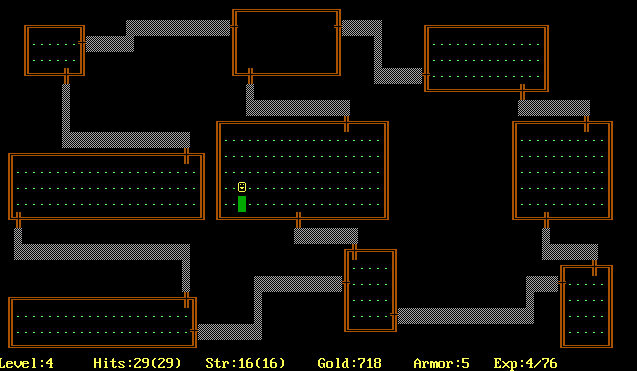
\includegraphics[width=0.9\textwidth]{Figuras/captura_3.png}
\caption{Captura de pantalla del videojuego original \textit{Rogue} (1980), mostrando la interfaz basada en caracteres ASCII y la disposición procedural de las salas. \textit{Fuente: captura histórica del juego.}}
\label{fig:placeholder-1}
\end{center}
\end{figure}


A lo largo de las décadas siguientes, numerosos títulos adoptaron y expandieron estas mecánicas. Juegos como \textit{NetHack} (1987), \textit{Angband} (1990) y \textit{Dungeon Crawl Stone Soup} (2006) mantuvieron la esencia del \textit{roguelike} clásico, caracterizado por gráficos basados en caracteres ASCII, mecánicas por turnos y una dificultad elevada. Sin embargo, a partir de la década de 2010, el subgénero experimentó una transformación significativa con la aparición de los denominados \textit{roguelites}, que incorporaban elementos del \textit{roguelike} clásico -- generación procedural y muerte permanente -- en combinación con mecánicas de acción en tiempo real, progresión entre partidas y diseño visual contemporáneo.

\subsection{Características técnicas fundamentales}


La comunidad de desarrolladores y jugadores ha intentado establecer criterios formales para definir qué constituye un \textit{roguelike}. La denominada \textit{Interpretación de Berlín} (International Roguelike Development Conference, 2008) \cite{BERLIN_INTERPRETATION} identificó las siguientes características como definitorias del subgénero:

\begin{enumerate}
\item \textbf{Generación procedural de niveles.} La estructura espacial del juego se genera algorítmicamente en cada partida, de modo que no existen dos ejecuciones idénticas. Esta característica implica la necesidad de diseñar algoritmos capaces de producir entornos jugables, coherentes y equilibrados sin intervención manual.
\item \textbf{Muerte permanente (\textit{permadeath}).} Al perder todos los puntos de vida, la partida finaliza de forma definitiva y el jugador debe reiniciar desde el principio. No existe la posibilidad de guardar y cargar el progreso del juego, lo que confiere a cada decisión del jugador un peso significativo.
\item \textbf{Progresión limitada a cada ejecución (\textit{run}, una partida completa desde el inicio hasta la muerte o victoria del jugador).} Las mejoras, armas y habilidades obtenidas durante una partida se pierden al morir. Cada ejecución comienza desde un estado inicial predefinido, aunque títulos más recientes (\textit{roguelites}) introducen sistemas de progresión permanente entre partidas.
\item \textbf{Sistema basado en turnos.} En la definición clásica, el jugador y los enemigos actúan de forma alternada. Sin embargo, los \textit{roguelikes} modernos y los \textit{roguelites} frecuentemente adoptan mecánicas de acción en tiempo real, como ocurre en el caso del proyecto \textit{Ascension}.
\item \textbf{Exploración de mazmorras (\textit{dungeon crawling}).} El jugador explora una sucesión de niveles o salas, enfrentándose a enemigos y recogiendo recursos, con el objetivo de alcanzar una condición de victoria definida.
\item \textbf{Alta rejugabilidad.} La combinación de generación procedural y la variabilidad de los elementos de juego (enemigos, objetos, disposición espacial) contribuye a que cada partida ofrezca una experiencia diferente, incentivando al jugador a repetir la experiencia.
\item \textbf{Complejidad de sistemas interconectados.} Los \textit{roguelikes} suelen presentar múltiples sistemas que interactúan entre sí de formas emergentes, generando situaciones impredecibles que enriquecen la experiencia de juego.
\end{enumerate}

\subsection{Importancia del género en la industria del videojuego}


El subgénero \textit{roguelike} ha experimentado un crecimiento notable en la última década, consolidándose como uno de los géneros más populares en el segmento de los videojuegos independientes. La amplia presencia de títulos etiquetados como \textit{roguelike} en catálogos de distribución digital refleja esta popularidad.

La relevancia del género se manifiesta en varios indicadores:

\begin{itemize}
\item \textbf{Éxito comercial.} Diversos títulos del subgénero han alcanzado un rendimiento comercial significativo, consolidándose como referencias dentro del mercado independiente.
\item \textbf{Reconocimiento crítico.} \textit{Hades} obtuvo reconocimiento en premios de la industria, incluyendo el premio al Mejor Juego Independiente en \textit{The Game Awards} 2020 \cite{CNET_GAME_AWARDS_2020_WINNERS}. Estos reconocimientos evidencian que el subgénero ha trascendido el ámbito de los juegos independientes para competir con producciones de mayor presupuesto.
\item \textbf{Influencia en el diseño de juegos.} Elementos propios del \textit{roguelike} -- generación procedural, \textit{permadeath}, rejugabilidad -- se han integrado en géneros distintos, dando lugar a híbridos como \textit{Returnal} (Housemarque, 2021), un juego de acción en tercera persona con estructura \textit{roguelike}, o \textit{Slay the Spire} (Mega Crit, 2019), que combina la estructura \textit{roguelike} con mecánicas de juegos de cartas \cite{STEAM_SLAY_THE_SPIRE_STORE}.
\item \textbf{Accesibilidad para desarrolladores independientes.} La generación procedural de contenido reduce la necesidad de diseño manual de niveles, lo que permite a equipos pequeños o desarrolladores individuales crear productos con una cantidad de contenido que, de otro modo, requeriría recursos significativamente mayores. Esta característica convierte al subgénero en un dominio adecuado para proyectos académicos como el presente Trabajo de Fin de Grado.
\end{itemize}

\begin{figure}[H]
\begin{center}
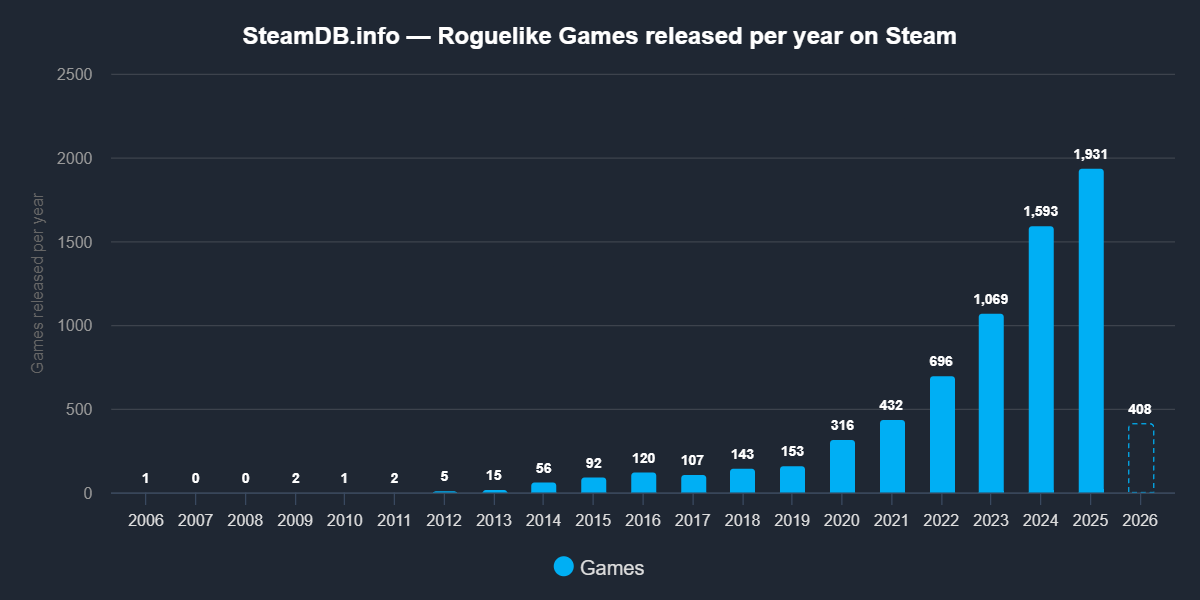
\includegraphics[width=0.9\textwidth]{Figuras/captura_4.png}
\caption{Gráfico que muestra la evolución del número de títulos \textit{roguelike} publicados en Steam por año (2006–2026). \textit{Fuente: SteamDB}}
\label{fig:placeholder-2}
\end{center}
\end{figure}


\subsection{Distinción entre \textit{roguelike} y \textit{roguelite}}


Resulta pertinente distinguir entre \textit{roguelike} en sentido estricto y \textit{roguelite}, dado que el proyecto \textit{Ascension} se sitúa en la intersección de ambas categorías:

\begin{table}[H]
\begin{center}
\small
\begin{tabular}{|p{0.307\textwidth}|p{0.307\textwidth}|p{0.307\textwidth}|}
\hline
\textbf{Característica} & \textbf{\textit{Roguelike} clásico} & \textbf{\textit{Roguelite}} \\ \hline
Generación procedural & Sí & Sí \\ \hline
Muerte permanente & Total & Total o parcial \\ \hline
Mecánica de combate & Por turnos & Tiempo real \\ \hline
Progresión entre partidas & No & Frecuente \\ \hline
Representación gráfica & ASCII o 2D simple & 2D/3D variada \\ \hline
Complejidad de sistemas & Muy alta & Moderada-alta \\ \hline
\end{tabular}
\end{center}
\end{table}


\TablaTitulo{Comparativa entre \textit{roguelike} clásico y \textit{roguelite}.}

\textit{Ascension} adopta las mecánicas fundamentales del \textit{roguelike} (generación procedural, \textit{permadeath}, exploración de mazmorras) con un sistema de combate en tiempo real propio del \textit{roguelite}, sin incluir progresión permanente entre partidas -- salvo la persistencia de puntuaciones -- lo que lo acerca más a la definición clásica del subgénero.

\subsection{Generación procedural de contenido}


La Generación Procedural de Contenido (GPC) constituye un conjunto de técnicas orientadas a la creación automática de datos de juego mediante algoritmos, reduciendo o eliminando la necesidad de diseño manual de niveles, escenarios o elementos del entorno (Shaker, Togelius y Nelson, 2016) \cite{SHAKER_PCG}.

En el contexto de los \textit{roguelikes}, la GPC resulta un componente central, ya que permite ofrecer variabilidad estructural y funcional en cada partida.

Entre los enfoques más utilizados para la generación procedural de niveles en videojuegos bidimensionales se encuentran:

\begin{itemize}
\item \textbf{Algoritmos basados en reglas.} Definen un conjunto de restricciones que deben cumplirse en el contenido generado (por ejemplo, que toda sala tenga al menos una salida accesible). El generador aplica estas reglas de forma iterativa hasta producir un resultado válido.
\item \textbf{Autómatas celulares.} Utilizados frecuentemente para la generación de cuevas orgánicas. Cada celda de una rejilla se evalúa según las celdas vecinas, produciendo formaciones naturales mediante iteraciones sucesivas.
\item \textbf{BSP (\textit{Binary Space Partitioning}).} Divide recursivamente el espacio disponible en subespacios menores, creando en cada subdivisión una habitación. Las habitaciones se conectan mediante pasillos, lo que genera estructuras de mazmorra clásicas.
\item \textbf{Sistemas deterministas con semillas pseudoaleatorias.} Utilizan un valor de semilla para inicializar el generador de números aleatorios, permitiendo reproducir exactamente la misma disposición espacial a partir de la misma semilla.
\item \textbf{Sistemas basados en \textit{Wave Function Collapse} (WFC).} Inspirados en la mecánica cuántica, definen restricciones de adyacencia entre tiles y resuelven iterativamente la disposición completa del nivel, produciendo resultados visualmente coherentes.
\item \textbf{Gramáticas formales y L-systems.} Utilizan reglas de producción para generar estructuras complejas a partir de axiomas simples, aplicados habitualmente a la generación de vegetación y elementos orgánicos.
\end{itemize}

En el caso de \textit{Ascension}, la generación procedural se basa en un enfoque híbrido: se utiliza una estructura rectangular fija de $26 \times 12$ tiles con bordes de muros perimetrales de un tile de grosor, sobre la cual se aplica un algoritmo de distribución aleatoria de tiles de suelo con variantes visuales y un algoritmo de expansión por \textit{clusters} para la colocación de tiles especiales con efectos.

La elección de este enfoque frente a técnicas más complejas como BSP o WFC se justifica por tres razones concretas. En primer lugar, la estructura rectangular fija simplifica el cálculo de posiciones válidas para la aparición de enemigos, ya que cualquier coordenada dentro del perímetro de muros constituye una posición válida sin necesidad de verificaciones adicionales de accesibilidad. En segundo lugar, los bordes perimetrales de muros impiden que el jugador pueda abandonar el área de juego sin necesidad de lógica de contención adicional; el colisionador del \textit{tilemap} de muros se genera automáticamente a partir de la posición de los tiles. En tercer lugar, el algoritmo de \textit{clusters} permite controlar la distribución espacial de los tiles especiales -- agrupándolos en manchas de entre cuatro y nueve tiles -- de forma que el jugador encuentre zonas con efectos lo suficientemente grandes como para influir en las decisiones tácticas de combate, pero no tan extensas como para dominar la sala. Este enfoque combina la previsibilidad estructural con la variabilidad de contenido que caracteriza al subgénero.

\subsubsection{Técnicas emergentes y trabajos recientes}


Además de los enfoques clásicos enumerados anteriormente, en los últimos años han surgido técnicas que amplían las posibilidades de la generación procedural en videojuegos:

\begin{itemize}
\item \textbf{Generación basada en restricciones con \textit{solvers} (Constraint Satisfaction Problems, CSP).} Formulan la generación de niveles como un problema de satisfacción de restricciones y emplean \textit{solvers} (como SAT o programación por restricciones) para encontrar configuraciones válidas que cumplan todas las condiciones impuestas. Smith y Mateas (2011) aplicaron esta técnica a la generación de niveles de plataformas 2D \cite{SMITH_MATEAS_2011}.
\item \textbf{Generación asistida por aprendizaje automático.} Se han explorado redes neuronales generativas (GANs -- \textit{Generative Adversarial Networks}) y autoencoders variacionales (VAEs -- \textit{Variational AutoEncoders}) para aprender la distribución de niveles diseñados manualmente y generar nuevos niveles consistentes con ese estilo (Volz et al., 2018) \cite{VOLZ_2018}.
\item \textbf{Funciones de ruido para generación de terreno.} Las funciones de ruido Perlin y Simplex, originalmente propuestas para la generación de texturas (Perlin, 1985) \cite{PERLIN_1985}, se utilizan ampliamente en juegos como \textit{Minecraft} y \textit{Terraria} para generar terrenos con apariencia natural.
\item \textbf{\textit{Wave Function Collapse} (WFC) aplicado a \textit{tilemaps}.} Gumin (2016) propuso el algoritmo WFC como un procedimiento genérico de generación a partir de ejemplos \cite{GUMIN_WFC_2016}. Karth y Smith (2017) analizaron formalmente el algoritmo y demostraron su equivalencia con ciertos modelos de propagación de restricciones \cite{KARTH_SMITH_2017}.
\end{itemize}

La siguiente tabla sintetiza la comparación entre las técnicas de generación procedural evaluadas y el enfoque adoptado en \textit{Ascension}:

\begin{table}[H]
\begin{center}
\small
\begin{tabular}{|p{0.23\textwidth}|p{0.23\textwidth}|p{0.23\textwidth}|p{0.23\textwidth}|}
\hline
\textbf{Técnica} & \textbf{Fortaleza principal} & \textbf{Limitación principal} & \textbf{Adecuación para \textit{Ascension}} \\ \hline
BSP & Salas irregulares con pasillos & Requiere verificación de accesibilidad & Baja: complejidad innecesaria para sala única \\ \hline
Autómatas celulares & Formas orgánicas (cuevas) & Difícil control de proporciones & Baja: salas rectangulares requeridas \\ \hline
WFC & Coherencia visual automática & Coste variable, reglas de adyacencia complejas & Moderada: sobrecomplejo para 8 tipos de tile \\ \hline
CSP / \textit{solvers} & Garantía de validez & Tiempo de cómputo elevado & Baja: no requiere verificación formal \\ \hline
GANs / VAEs & Captura de estilos implícitos & Requiere datos de entrenamiento, sin garantía & Baja: sin corpus de niveles previo \\ \hline
Ruido Perlin/Simplex & Terrenos naturales continuos & No discreto, sin control de salas & Baja: generación por tiles, no continua \\ \hline
Rejilla fija + \textit{clusters} & Control total, posicionamiento simple & Geometría invariante & Alta: equilibrio complejidad/variabilidad \\ \hline
\end{tabular}
\end{center}
\end{table}


\TablaTitulo{Comparativa de técnicas de generación procedural y su adecuación al proyecto.}

La tabla evidencia que, para un proyecto con sala rectangular fija, tres tipos de enemigo y un sistema de tiles con efectos como fuente principal de variabilidad, las técnicas más sofisticadas habrían incrementado la complejidad de implementación sin producir un beneficio proporcional en la experiencia de juego. La variabilidad táctica de \textit{Ascension} reside en la composición de tiles con efectos y en la combinación de oleadas de enemigos, no en la forma geométrica de la sala.

\subsection{Inteligencia artificial en videojuegos 2D}


La Inteligencia Artificial (IA) en videojuegos bidimensionales se orienta al diseño de comportamientos creíbles y coherentes para los Personajes No Jugables (PNJ) (Millington y Funge, 2009) \cite{MILLINGTON_AI}.

Las técnicas más empleadas para la implementación de IA en videojuegos incluyen:

\begin{itemize}
\item \textbf{Máquinas de estados finitos (FSM).} Definen un conjunto discreto de estados posibles para un PNJ y las condiciones que provocan la transición entre estados. Son fáciles de implementar y de depurar, pero pueden resultar rígidas cuando el número de estados crece.
\item \textbf{Árboles de comportamiento (\textit{behavior trees}).} Estructuran la lógica de decisión en forma de árbol jerárquico, donde cada nodo representa una condición, una acción o una secuencia de acciones.
\item \textbf{Sistemas de decisión basados en reglas.} Evalúan un conjunto de condiciones y ejecutan la acción asociada a la regla de mayor prioridad que se cumpla.
\item \textbf{Navegación por mallas (\textit{navmesh}) y \textit{pathfinding}.} Algoritmos como A* o Dijkstra permiten calcular rutas óptimas entre dos puntos del nivel.
\item \textbf{Sistemas de utilidad (\textit{Utility AI}).} Evalúan numéricamente la utilidad de cada acción disponible en función del estado actual del mundo.
\item \textbf{\textit{Goal-Oriented Action Planning} (GOAP).} Los agentes definen objetivos y planifican secuencias de acciones para alcanzarlos. Orkin (2003) introdujo GOAP en \textit{F.E.A.R.} \cite{ORKIN_2003}.
\item \textbf{Aprendizaje por refuerzo.} Los agentes aprenden comportamientos óptimos mediante la maximización de una función de recompensa. Unity ML-Agents (Juliani et al., 2018) \cite{JULIANI_2018} proporciona un \textit{framework} -- un entorno de desarrollo con herramientas y bibliotecas predefinidas -- integrado para entrenar agentes mediante aprendizaje por refuerzo profundo (DRL, \textit{Deep Reinforcement Learning}).
\end{itemize}

En \textit{Ascension}, la inteligencia artificial de los enemigos se implementa mediante una combinación de máquinas de estados simples y sistemas de decisión basados en reglas, cuya justificación se detalla en la siguiente tabla comparativa:

\begin{table}[H]
\begin{center}
\small
\begin{tabular}{|p{0.17\textwidth}|p{0.17\textwidth}|p{0.17\textwidth}|p{0.17\textwidth}|p{0.17\textwidth}|}
\hline
\textbf{Técnica} & \textbf{Complejidad de implementación} & \textbf{Expresividad} & \textbf{Depurabilidad} & \textbf{Adecuación para 3 tipos de enemigo} \\ \hline
FSM & Baja & Moderada & Alta (estados discretos) & Alta \\ \hline
Árboles de comportamiento & Moderada & Alta & Moderada (nodos jerárquicos) & Moderada \\ \hline
Sistemas de utilidad & Moderada-alta & Alta & Baja (valores continuos) & Baja \\ \hline
GOAP & Alta & Muy alta & Baja (planes dinámicos) & Baja \\ \hline
Aprendizaje por refuerzo & Muy alta & Variable & Muy baja (caja negra) & Muy baja \\ \hline
\end{tabular}
\end{center}
\end{table}


\TablaTitulo{Comparativa de técnicas de IA para enemigos en videojuegos 2D.}

\subsection{Mecánicas de combate en \textit{roguelikes}}


El sistema de combate constituye una de las mecánicas centrales de los videojuegos \textit{roguelike} y \textit{roguelite}. Los enfoques más habituales incluyen:

\begin{itemize}
\item \textbf{Combate por turnos.} El jugador y los enemigos ejecutan acciones de forma alternada. Es el enfoque clásico del subgénero (\textit{Rogue}, \textit{NetHack}).
\item \textbf{Combate en tiempo real con \textit{hack and slash} (combate de acción basado en ataques cuerpo a cuerpo rápidos y encadenados).} El jugador controla el personaje en tiempo real, ejecutando ataques de forma continua. Ejemplos representativos incluyen \textit{Hades} y \textit{Dead Cells}.
\item \textbf{Combate en tiempo real con componente de disparos (\textit{top-down shooter}).} El jugador dispara proyectiles hacia los enemigos desde una perspectiva cenital. Títulos como \textit{The Binding of Isaac} y \textit{Enter the Gungeon} han popularizado este enfoque.
\item \textbf{Combate híbrido.} Combina armas cuerpo a cuerpo y a distancia, permitiendo al jugador alternar entre estilos según la situación. \textit{Ascension} adopta este enfoque, ofreciendo ambas modalidades de combate con mecánicas diferenciadas.
\end{itemize}

\section{Análisis de mercado: referencias comerciales del subgénero}


El diseño y desarrollo de \textit{Ascension} se ha llevado a cabo tomando como referencia una selección de títulos comerciales representativos del subgénero \textit{roguelike} y \textit{roguelite}. El estudio de estos productos ha permitido identificar mecánicas de juego, decisiones de diseño y patrones de interacción que han influido en la definición de los sistemas del proyecto. A continuación se analizan los títulos más relevantes.

\subsection{The Binding of Isaac (2011, Edmund McMillen)}


\textit{The Binding of Isaac} es un \textit{roguelike} con perspectiva cenital (\textit{top-down}) cuya mecánica de combate se basa en el disparo de proyectiles en las cuatro direcciones cardinales. El jugador explora una sucesión de salas generadas proceduralmente, enfrentándose a enemigos con patrones de movimiento y ataque variados.

\textbf{Características relevantes para \textit{Ascension}:}
\begin{itemize}
\item \textbf{Estructura de salas.} Cada sala constituye un espacio cerrado con enemigos que deben ser derrotados antes de poder avanzar. En \textit{The Binding of Isaac}, las puertas de la sala se cierran al entrar y se abren al completarla. En \textit{Ascension}, la progresión se representa mediante escaleras que se bloquean durante el combate y se habilitan al completar la sala.
\item \textbf{Vista cenital.} La perspectiva \textit{top-down} permite al jugador una visión completa de la sala, facilitando la planificación táctica del movimiento y el combate. \textit{Ascension} utiliza esta misma perspectiva.
\item \textbf{Variedad de enemigos.} Cada tipo de enemigo presenta un comportamiento diferenciado (persecución, disparo, movimiento errático), lo que obliga al jugador a adaptar su estrategia continuamente.
\item \textbf{Sistema de jefes periódicos.} Al final de cada piso, el jugador se enfrenta a un enemigo jefe con estadísticas superiores y mecánicas de ataque propias. \textit{Ascension} implementa un sistema análogo con jefes cada cinco salas.
\end{itemize}

\begin{figure}[htbp]
\begin{center}
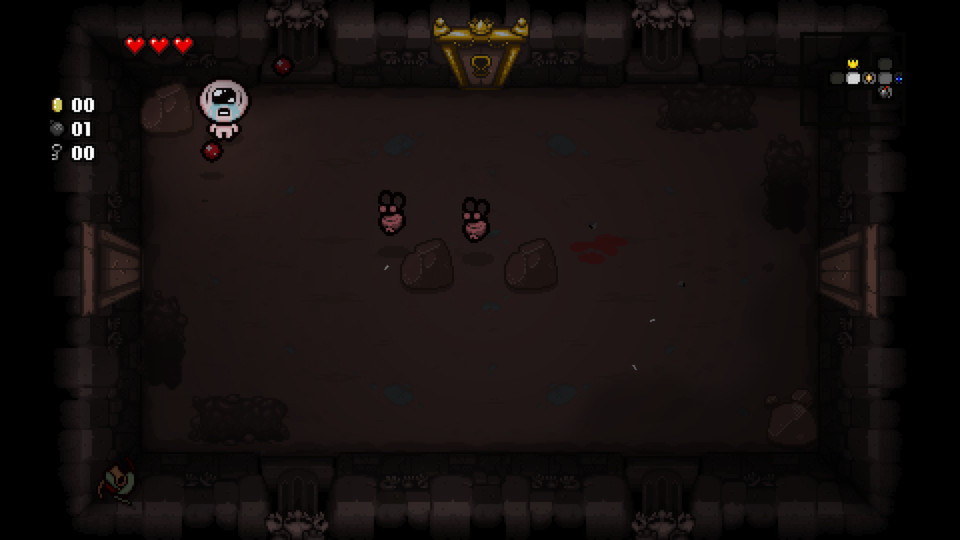
\includegraphics[width=0.9\textwidth]{Figuras/captura_5.png}
\caption{Captura de pantalla de \textit{The Binding of Isaac: Rebirth} en la que se observa la perspectiva cenital, la estructura de sala cerrada con puertas y la interfaz de vida mediante corazones en la esquina superior izquierda. \textit{Fuente: captura del juego en Steam.}}
\label{fig:placeholder-3}
\end{center}
\end{figure}


\subsection{Enter the Gungeon (2016, Dodge Roll)}


\textit{Enter the Gungeon} es un \textit{roguelite} cenital centrado en el combate con armas de fuego. Destaca por su sistema de esquiva (\textit{dodge roll}) y por la amplia variedad de armas disponibles, cada una con mecánicas diferenciadas.

\textbf{Características relevantes para \textit{Ascension}:}
\begin{itemize}
\item \textbf{Mecánica de esquiva (\textit{roll}).} El jugador puede ejecutar un movimiento rápido con invulnerabilidad temporal para evitar el daño de los proyectiles enemigos. \textit{Ascension} implementa una mecánica de esquiva equivalente, activada mediante la tecla Espacio, con un periodo de invulnerabilidad y un tiempo de espera entre usos.
\item \textbf{Combinación de combate a distancia y cuerpo a cuerpo.} \textit{Ascension} ofrece ambas modalidades de combate como mecánicas diferenciadas asociadas a tipos de arma distintos.
\item \textbf{Generación procedural con estructura por pisos.} El juego genera cada piso de la mazmorra de forma procedural. \textit{Ascension} adopta una estructura en la que se genera proceduralmente el contenido de la sala.
\end{itemize}

\begin{figure}[H]
\begin{center}
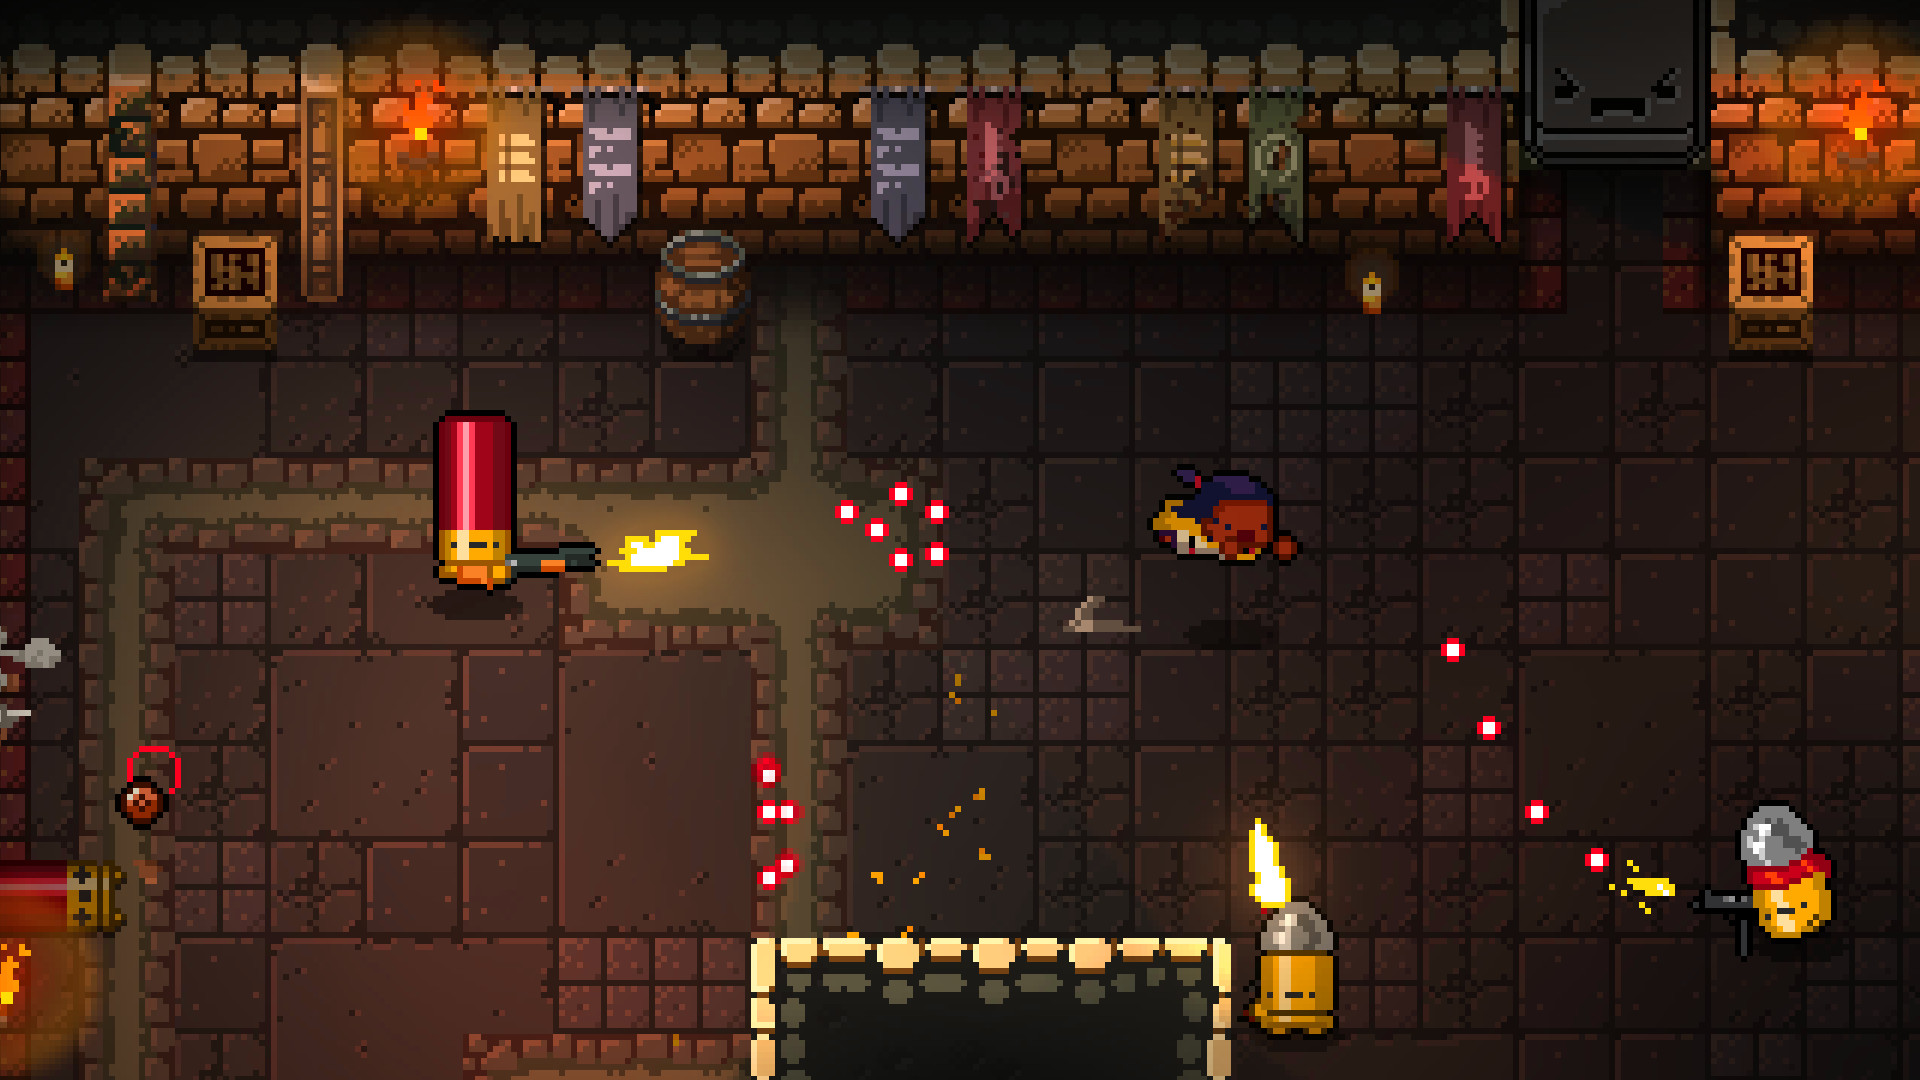
\includegraphics[width=0.9\textwidth]{Figuras/captura_6.png}
\caption{Captura de pantalla de \textit{Enter the Gungeon} en la que se muestra la mecánica de esquiva (\textit{dodge roll}) durante el combate y la variedad de proyectiles en pantalla. \textit{Fuente: captura del juego en Steam.}}
\label{fig:placeholder-4}
\end{center}
\end{figure}


\subsection{Hades (2020, Supergiant Games)}


\textit{Hades} es un \textit{roguelite} de acción con perspectiva isométrica que combina combate rápido con una narrativa progresiva. Ha recibido reconocimiento en premios de la industria; por ejemplo, en \textit{The Game Awards} 2020 obtuvo el galardón a Mejor Juego Independiente \cite{CNET_GAME_AWARDS_2020_WINNERS}.

\textbf{Características relevantes para \textit{Ascension}:}
\begin{itemize}
\item \textbf{Variedad de armas con mecánicas únicas.} Cada arma presenta un estilo de combate diferenciado (espada, arco, escudo, lanza). \textit{Ascension} implementa armas cuerpo a cuerpo y a distancia con mecánicas de ataque diferenciadas.
\item \textbf{Sistema de clases de personaje.} Aunque en \textit{Hades} no existen clases como tales, la selección de arma al inicio de cada ejecución determina el estilo de juego. \textit{Ascension} formaliza este concepto mediante un sistema de selección de clase con estadísticas diferenciadas.
\item \textbf{Enemigos con comportamientos variados.} Los enemigos presentan patrones de ataque diferenciados y coordinados. \textit{Ascension} implementa esta variedad mediante tres tipos de enemigos con comportamientos específicos.
\item \textbf{Retroalimentación visual del combate.} \textit{Hades} destaca por la retroalimentación visual que proporciona al jugador. \textit{Ascension} incorpora mecanismos análogos como el parpadeo en blanco del jugador al recibir daño y un parpadeo rojo rápido tanto en enemigos como en el jugador justo antes de morir.
\end{itemize}

\begin{figure}[H]
\begin{center}
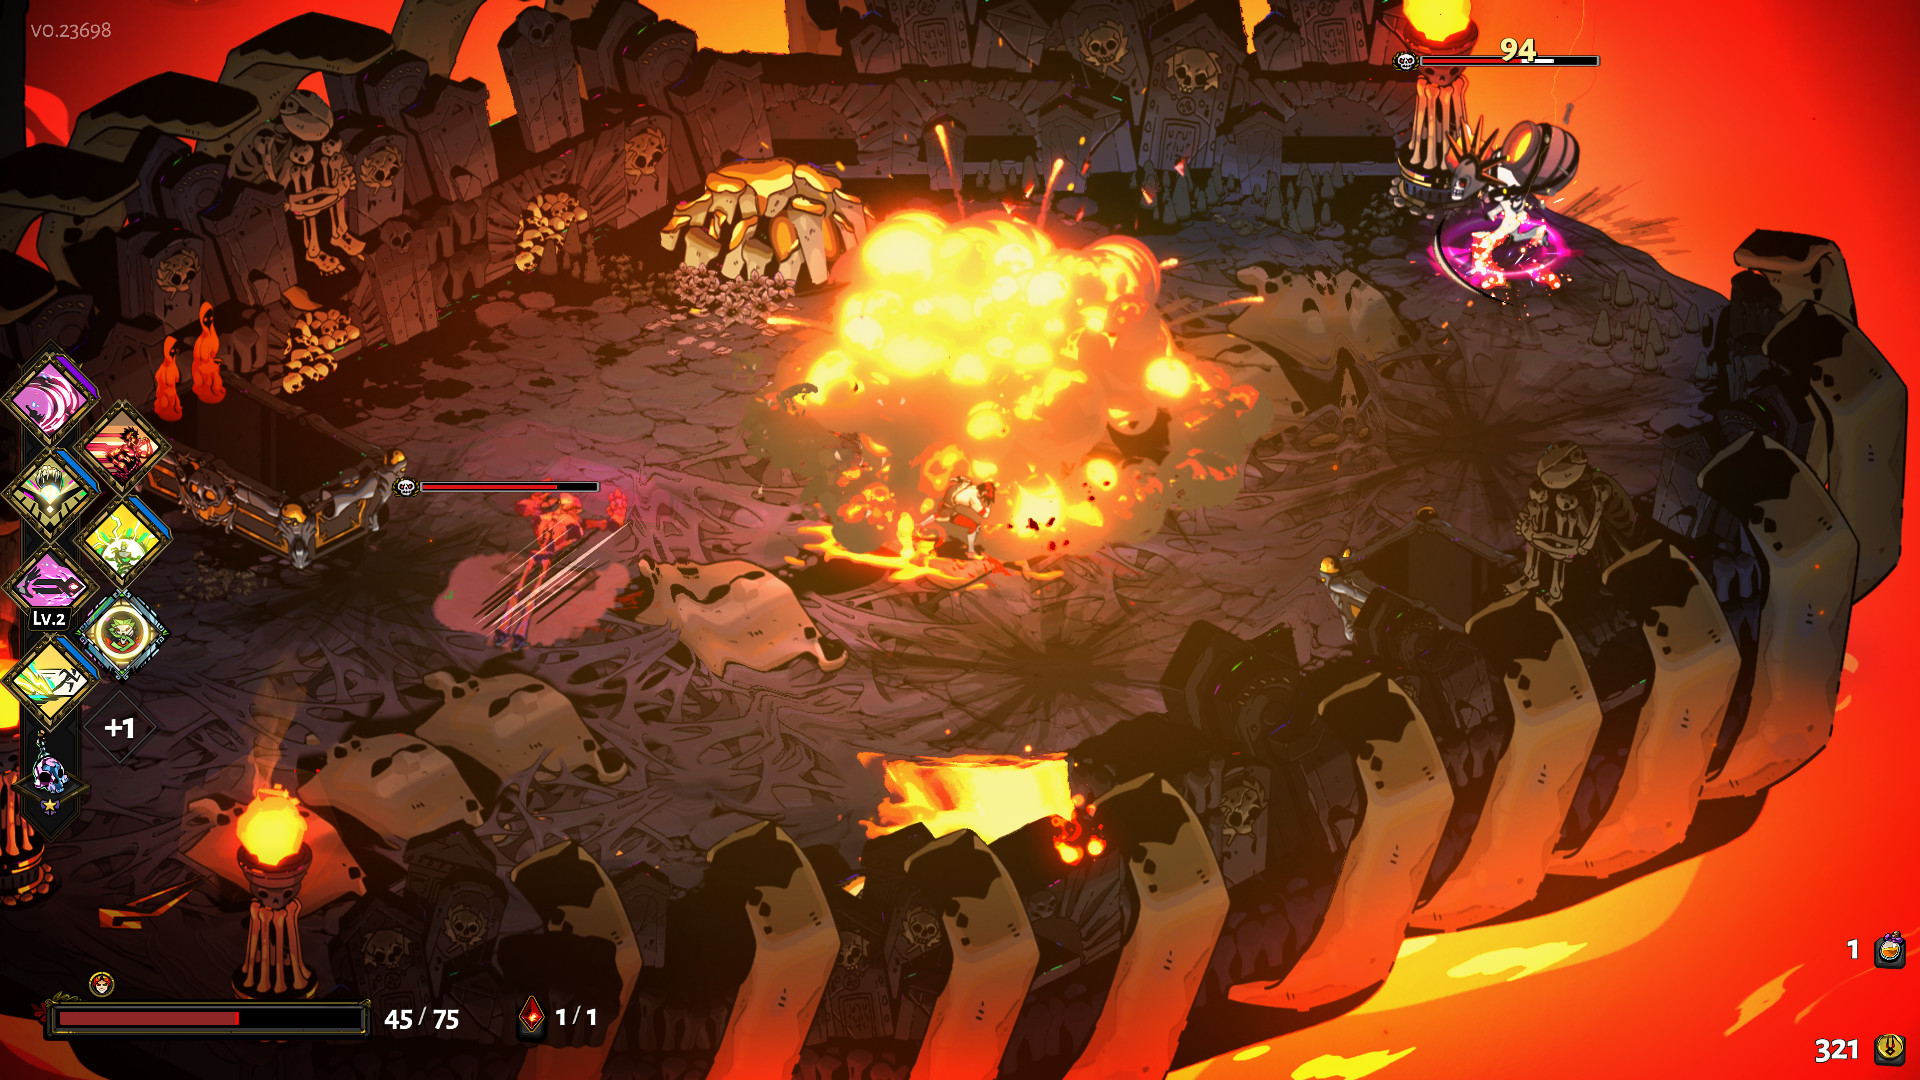
\includegraphics[width=0.9\textwidth]{Figuras/captura_7.png}
\caption{Captura de pantalla de \textit{Hades} en la que se aprecia el sistema de combate en tiempo real con arma cuerpo a cuerpo, la variedad de enemigos simultáneos y la interfaz de estado del personaje. \textit{Fuente: captura del juego en Steam.}}
\label{fig:placeholder-5}
\end{center}
\end{figure}


\subsection{Dead Cells (2018, Motion Twin)}


\textit{Dead Cells} es un \textit{roguelite} de acción lateral (\textit{side-scroller}) que combina exploración, combate fluido y un sistema de progresión permanente entre partidas.

\textbf{Características relevantes para \textit{Ascension}:}
\begin{itemize}
\item \textbf{Combate ágil y responsivo.} \textit{Dead Cells} se caracteriza por un combate rápido y preciso. En \textit{Ascension} se han implementado controles responsivos y tiempos de espera (\textit{cooldown}) reducidos con el objetivo de aproximarse a este enfoque.
\item \textbf{Armas con comportamientos diferenciados.} El juego ofrece una amplia variedad de armas cuerpo a cuerpo y a distancia. \textit{Ascension} implementa esta distinción mediante las clases \texttt{MeleeWeapon} y \texttt{RangedWeapon}, aplicando el patrón \textit{Strategy}.
\item \textbf{Escalonamiento de dificultad.} La dificultad aumenta de forma progresiva. En \textit{Ascension}, la dificultad se incrementa mediante el aumento del presupuesto de coste de enemigos por sala y la aparición periódica de enemigos especiales con atributos escalados.
\end{itemize}

En este contexto, el término \textit{cooldown} se refiere al \textbf{tiempo mínimo de espera entre dos ejecuciones de una misma acción} (por ejemplo, entre dos ataques consecutivos), y se utiliza como mecanismo de equilibrado para evitar acciones excesivamente frecuentes.

\begin{figure}[H]
\begin{center}
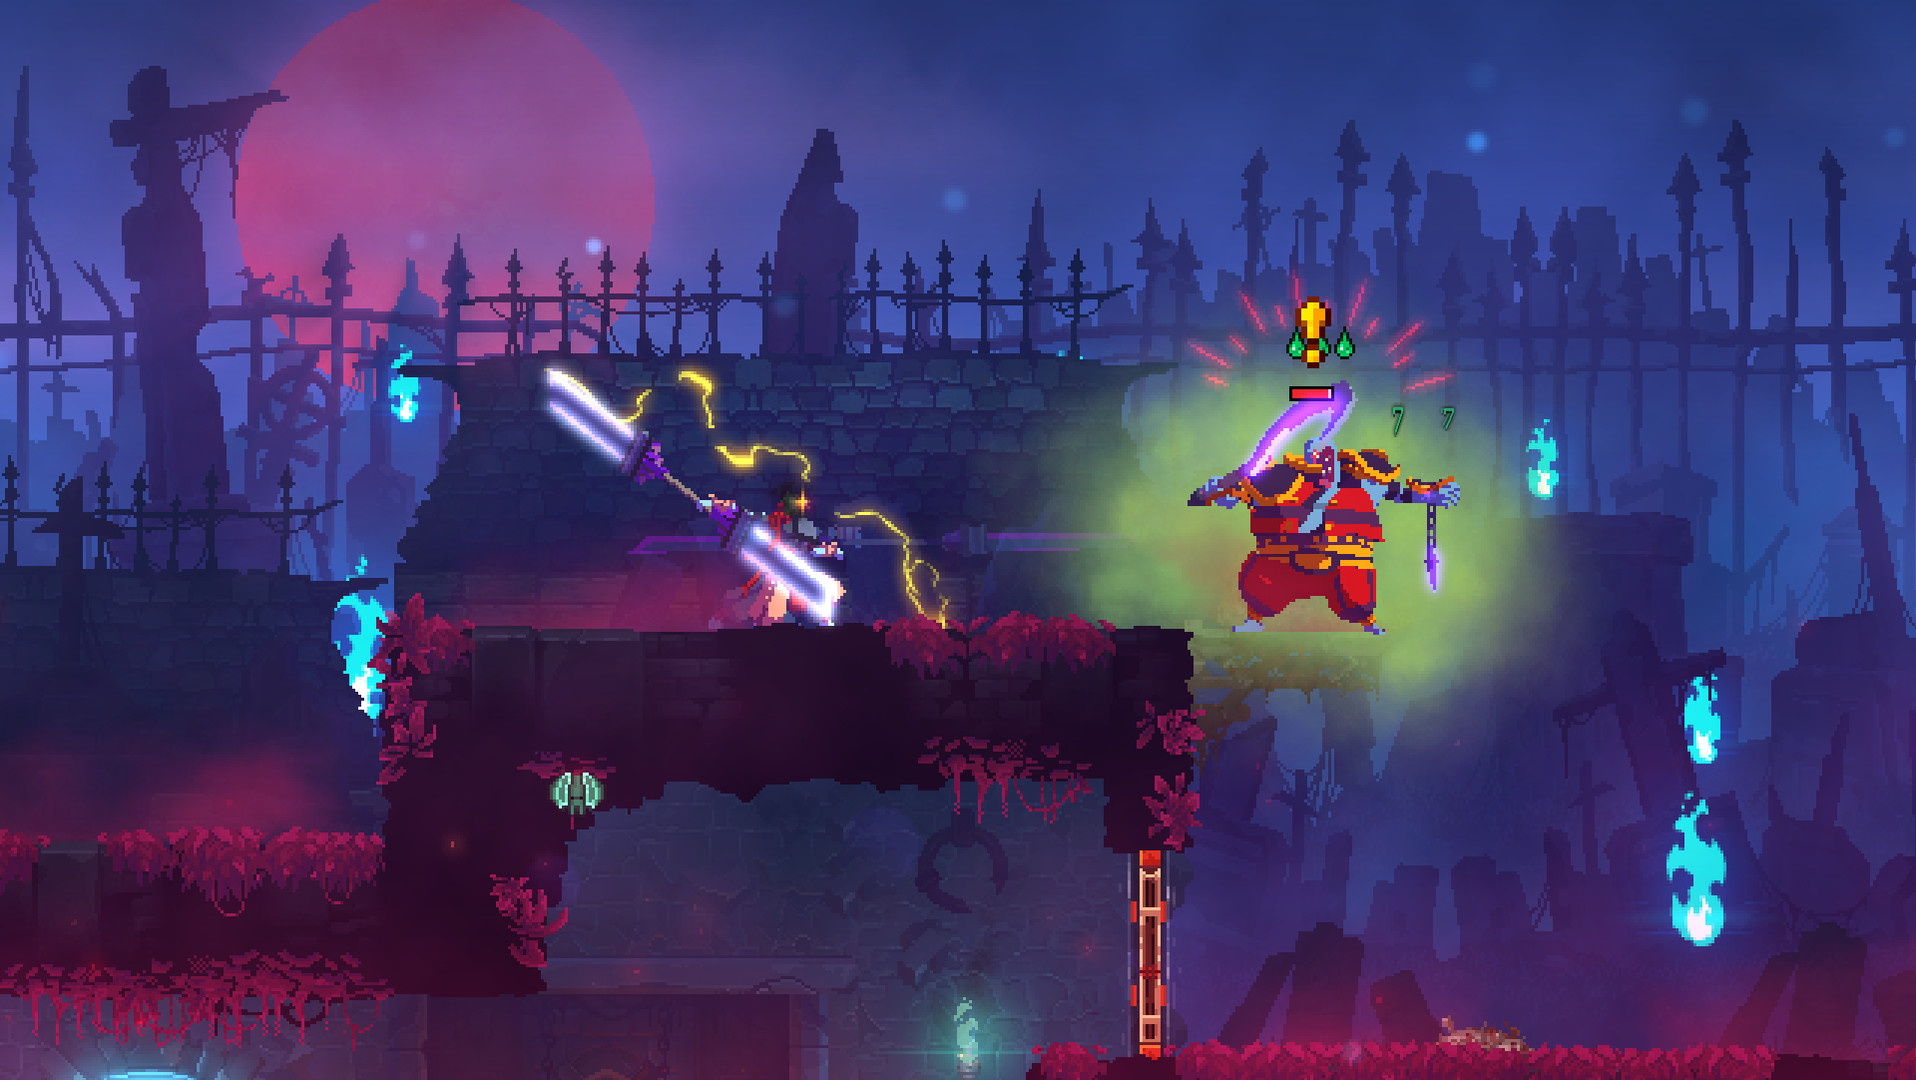
\includegraphics[width=0.9\textwidth]{Figuras/captura_8.png}
\caption{Captura de pantalla de \textit{Dead Cells} en la que se observa el combate lateral con armas cuerpo a cuerpo. \textit{Fuente: captura del juego en Steam.}}
\label{fig:placeholder-6}
\end{center}
\end{figure}


\subsection{Tabla comparativa de referencias comerciales}

La siguiente tabla compara las características de diseño y tecnología de los referentes analizados frente a \textit{Ascension}, justificando las decisiones adoptadas en cuanto a perspectiva, combate y mecánicas de movimiento.
\begin{table}[H]
\begin{center}
\small
\begin{tabular}{|p{0.153\textwidth}|p{0.153\textwidth}|p{0.153\textwidth}|p{0.153\textwidth}|p{0.153\textwidth}|p{0.153\textwidth}|}
\hline
Característica & The Binding of Isaac & Enter the Gungeon & Hades & Dead Cells & \textbf{Ascension} \\ \hline
Perspectiva & Cenital & Cenital & Isométrica & Lateral & \textbf{Cenital} \\ \hline
Generación procedural & Salas conectadas & Pisos con salas & Salas conectadas & Niveles laterales & \textbf{Salas secuenciales} \\ \hline
Combate & Disparo 4 direcciones & Disparo 360° + esquiva & Melee + distancia & Melee + distancia & \textbf{Melee + distancia} \\ \hline
Esquiva & No & \textit{Dodge roll} & \textit{Dash} & \textit{Roll} & \textbf{\textit{Roll} con invulnerabilidad} \\ \hline
Selección de personaje & Múltiples personajes & Múltiples personajes & Arma inicial & No & \textbf{3 clases con stats} \\ \hline
\textit{Permadeath} & Sí & Sí & Sí (con progresión) & Sí (con progresión) & \textbf{Sí} \\ \hline
Sistema de jefes & Final de piso & Final de piso & Final de zona & Por bioma & \textbf{Cada 5 salas} \\ \hline
Tiles con efectos & No & No & No & No & \textbf{Sí (hielo, lodo, curación, daño)} \\ \hline
Motor & Flash / C++ custom & Unity & Supergiant Engine & Custom & \textbf{Unity} \\ \hline
\end{tabular}
\end{center}
\end{table}


\TablaTitulo{Comparativa entre referencias comerciales y el proyecto \textit{Ascension}.}

\subsection{Elementos diferenciadores de \textit{Ascension}}


A partir del análisis comparativo anterior, es posible identificar los elementos que diferencian a \textit{Ascension} respecto a las referencias comerciales estudiadas:

\begin{enumerate}
\item \textbf{Sistema de tiles con efectos.} Ninguno de los títulos analizados incorpora un sistema de tiles especiales que modifiquen las condiciones de combate en tiempo real. Se incorporó este sistema en \textit{Ascension} para resolver un problema de diseño concreto: en un \textit{roguelike} con tres tipos de enemigo y un repertorio limitado de armas, la variabilidad táctica de cada sala depende exclusivamente de la composición de la oleada de enemigos, lo que puede generar repetitividad. Los tiles con efectos -- hielo (incremento de velocidad), lodo (reducción de velocidad), curación y potenciación de daño -- introducen una segunda dimensión de variabilidad: el entorno físico de la sala condiciona las decisiones tácticas del jugador. La alternativa descartada era añadir más tipos de enemigo, pero esto habría incrementado significativamente el volumen de arte y animación necesario.
\item \textbf{Arquitectura orientada a la extensibilidad.} Se adoptó la separación entre datos configurables (\textit{ScriptableObjects}) y lógica de juego como principio arquitectónico deliberado. Esta decisión responde a una necesidad práctica del desarrollo: los parámetros de configuración se modificaron en numerosas ocasiones. Con \textit{ScriptableObjects}, cada ajuste se realiza editando un campo numérico en el inspector, con efecto inmediato y sin recompilación. La implicación arquitectónica es que el sistema cumple el principio de apertura-cierre (\textit{Open-Closed Principle}) de los principios SOLID.
\end{enumerate}

\begin{figure}[H]
\begin{center}
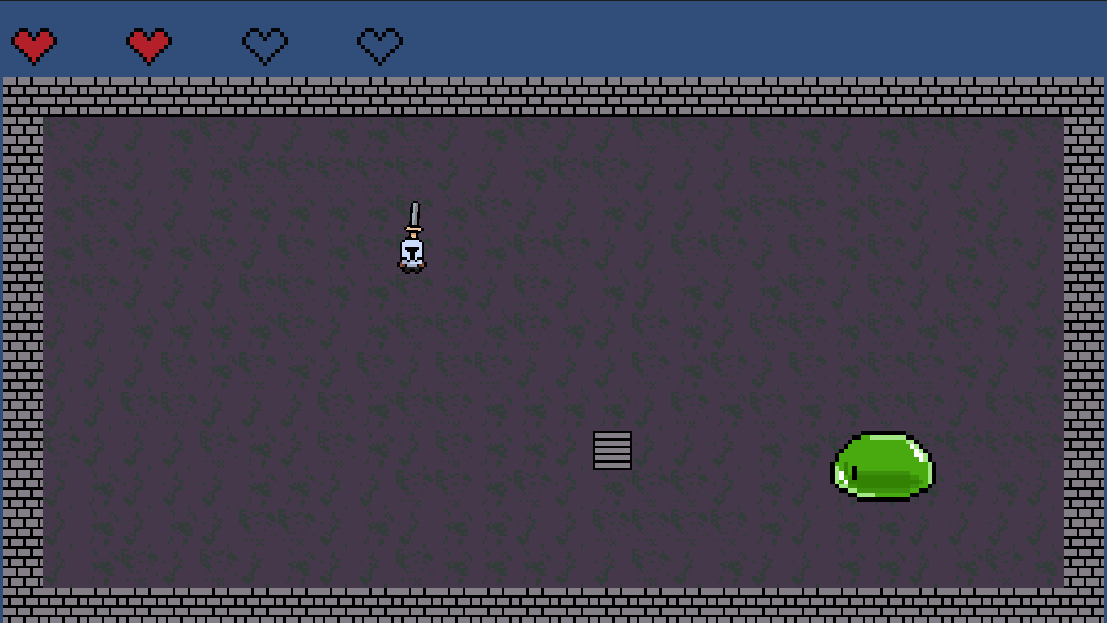
\includegraphics[width=0.9\textwidth]{Figuras/Jefe.png}
\caption{Captura de pantalla de \textit{Ascension} durante una partida, mostrando la perspectiva cenital, la sala generada proceduralmente con tiles especiales visibles (hielo, lodo), enemigos activos y la interfaz de corazones. \textit{Elaboración propia.}}
\label{fig:placeholder-7}
\end{center}
\end{figure}


\begin{figure}[H]
\begin{center}
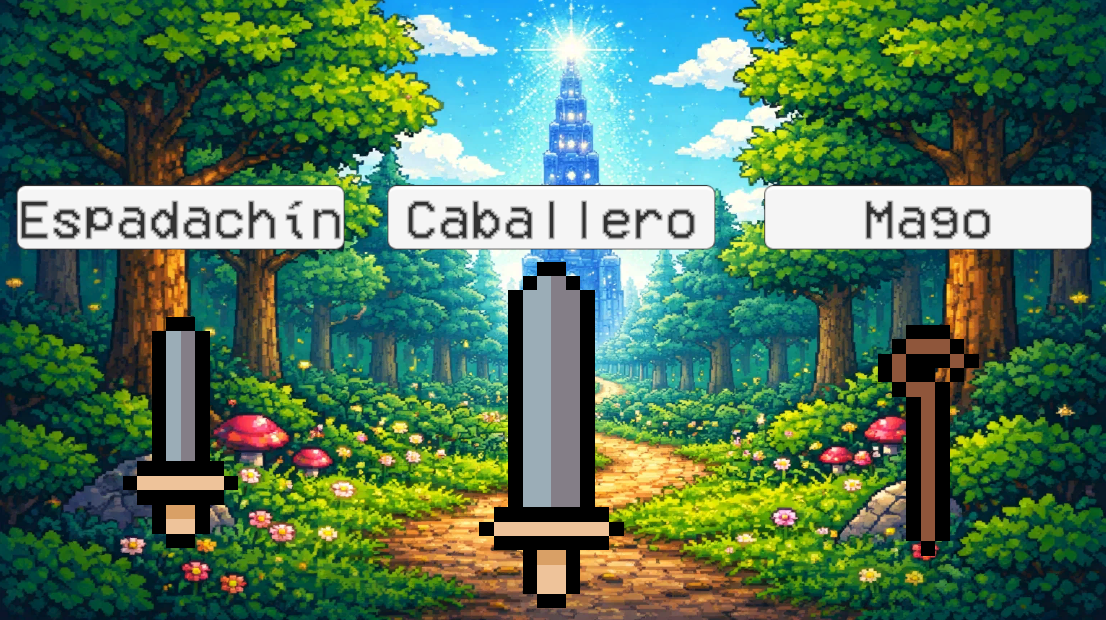
\includegraphics[width=0.9\textwidth]{Figuras/captura_1.png}
\caption{Captura de pantalla de \textit{Ascension} mostrando la pantalla de selección de clase. \textit{Elaboración propia.}}
\label{fig:placeholder-8}
\end{center}
\end{figure}




\section{Análisis de herramientas y tecnologías}


\subsection{Motores de desarrollo de videojuegos}


La selección del motor de desarrollo constituye una decisión técnica de gran relevancia en cualquier proyecto de videojuegos. A continuación se analizan los motores más relevantes para el desarrollo de videojuegos bidimensionales.

\subsubsection{Unity}


Unity es un motor de desarrollo multiplataforma creado por Unity Technologies en 2005. Constituye una de las herramientas más utilizadas en la industria; Unity indica que más del 70\% de los 1.000 juegos móviles más populares se desarrollaron con Unity (dato referido a Q4 2022 con fuente Apptopia) \cite{UNITY_MOBILE_TOP1000_APPTOPIA_Q4_2022}. Sus características principales incluyen:

\begin{itemize}
\item \textbf{Arquitectura basada en componentes (\textit{Entity-Component System}).} Las entidades del juego se definen como agregaciones de componentes reutilizables.
\item \textbf{Sistema de \textit{Tilemaps} integrado.} Proporciona herramientas nativas para la creación y gestión de niveles basados en tiles, incluyendo colisionadores automáticos.
\item \textbf{Lenguaje de programación C\#.} Ofrece tipado fuerte, soporte completo para programación orientada a objetos y acceso a la biblioteca estándar de .NET.
\item \textbf{Sistema de \textit{ScriptableObjects}.} Permite almacenar datos configurables como activos del proyecto.
\item \textbf{Soporte multiplataforma.} Permite compilar el proyecto para más de veinte plataformas.
\item \textbf{Comunidad y recursos.} Cuenta con documentación oficial detallada, foros activos y un amplio ecosistema de \textit{assets}.
\end{itemize}

\subsubsection{Godot Engine}


Godot es un motor de código abierto creado por Juan Linietsky y Ariel Manzur, publicado bajo licencia MIT. Sus características incluyen:

\begin{itemize}
\item \textbf{Arquitectura basada en nodos y escenas.} Toda entidad es un nodo dentro de un árbol de escenas.
\item \textbf{Lenguaje GDScript.} Lenguaje propio con sintaxis similar a Python. También soporta C\# y C++.
\item \textbf{Código abierto.} Permite acceder y modificar el código fuente del motor.
\item \textbf{Sistema de \textit{TileMap} y \textit{TileSet}.} Proporciona herramientas para el diseño de niveles 2D.
\item \textbf{Sin costes de licencia.}
\end{itemize}

\subsubsection{Unreal Engine}


Unreal Engine, desarrollado por Epic Games, es un motor enfocado principalmente en gráficos de alta fidelidad para juegos 3D AAA:

\begin{itemize}
\item \textbf{Sistema \textit{Blueprints}.} Permite programar mediante un sistema de scripting visual.
\item \textbf{Lenguaje C++.} Ofrece rendimiento nativo y control de bajo nivel.
\item \textbf{Orientación principal a 3D.} Carece de herramientas nativas específicas como \textit{tilemaps}.
\item \textbf{Peso del editor.} El editor tiene un tamaño considerable (más de 60 GB).
\end{itemize}

\subsubsection{GameMaker}


GameMaker, desarrollado por YoYo Games, es un motor orientado al desarrollo de videojuegos 2D:

\begin{itemize}
\item \textbf{Lenguaje GML (\textit{GameMaker Language}).} Orientado a la simplicidad.
\item \textbf{Especialización en 2D.} Herramientas nativas optimizadas para la creación de juegos bidimensionales.
\item \textbf{Limitaciones en proyectos complejos.} Arquitectura menos flexible para proyectos con requerimientos de modularidad avanzada.
\item \textbf{Licencia de pago.}
\end{itemize}

\subsection{Tabla comparativa de motores de desarrollo}

La elección del motor de desarrollo es un factor crítico para el éxito del proyecto. La siguiente tabla evalúa las alternativas más relevantes del mercado, comparando criterios técnicos clave —como el soporte nativo 2D y la gestión de datos— para justificar la idoneidad de la tecnología seleccionada para Ascension.

\begin{table}[H]
\begin{center}
\small
\begin{tabular}{|p{0.184\textwidth}|p{0.184\textwidth}|p{0.184\textwidth}|p{0.184\textwidth}|p{0.184\textwidth}|}
\hline
\textbf{Criterio} & \textbf{Unity} & \textbf{Godot} & \textbf{Unreal Engine} & \textbf{GameMaker} \\ \hline
Licencia & Gratuito (con restricciones) & MIT (libre) & Gratuito (regalías al 5 \%) & Pago \\ \hline
Lenguaje principal & C\# & GDScript / C\# & C++ / Blueprints & GML \\ \hline
Soporte 2D nativo & Excelente & Bueno & Limitado & Excelente \\ \hline
Sistema de \textit{Tilemaps} & Integrado y maduro & Integrado (Godot 4) & No nativo & Integrado \\ \hline
\textit{ScriptableObjects} & Sí & Recursos equivalentes & \textit{Data Assets} & No \\ \hline
Documentación y comunidad & Muy amplia & Creciente & Amplia (centrada en 3D) & Moderada \\ \hline
Soporte multiplataforma & +20 plataformas & +10 plataformas & +10 plataformas & +10 plataformas \\ \hline
Curva de aprendizaje & Moderada & Baja-moderada & Alta & Baja \\ \hline
Idoneidad para \textit{roguelikes} 2D & Alta & Alta & Baja & Moderada \\ \hline
\end{tabular}
\end{center}
\end{table}


\TablaTitulo{Comparativa de motores de desarrollo de videojuegos.}

\subsection{Justificación de la elección de Unity y C\#}


Se seleccionó Unity frente a Godot, Unreal Engine y GameMaker tras evaluar los criterios recogidos en la Tabla 2.5. La decisión se basa en cuatro requisitos técnicos concretos del proyecto:

\begin{enumerate}
\item \textbf{Madurez del sistema de \textit{Tilemaps}.} La generación procedural de salas basada en \textit{tilemaps} constituye una funcionalidad central del proyecto. El componente \texttt{TilemapCollider2D} de Unity genera colisionadores de forma nativa a partir de la disposición de tiles, mientras que en Godot la creación de colisionadores por tile requería configuración manual adicional.
\item \textbf{Sistema de \textit{ScriptableObjects}.} Resuelve un problema arquitectónico concreto: la separación entre datos configurables y lógica de ejecución. Sin este mecanismo, ajustar un parámetro de equilibrado obligaría a recompilar el proyecto.
\item \textbf{Lenguaje C\#.} Ofrece tipado fuerte, soporte completo para programación orientada a objetos (herencia, polimorfismo, interfaces), manejo de excepciones, eventos y delegados. Estas características resultan fundamentales para la implementación de patrones de diseño como \textit{Singleton}, \textit{Observer} y \textit{Strategy}.
\item \textbf{Documentación y soporte.} La documentación oficial de Unity, los foros de la comunidad y la abundancia de recursos formativos facilitan la resolución de problemas técnicos de forma autónoma.
\end{enumerate}

\subsection{Correspondencia entre funcionalidades de Unity/C\# y subsistemas del proyecto}


La implementación de los subsistemas en Ascension depende de características específicas del motor y del lenguaje C\#. La siguiente tabla detalla estas funcionalidades y su equivalencia en motores alternativos, permitiendo comprender cómo la arquitectura del proyecto -- basada en patrones como Observer o Strategy -- se ve favorecida por las herramientas nativas de Unity.


\begin{table}[H]
\begin{center}
\scriptsize
\setlength{\tabcolsep}{2pt}
\begin{tabular}{|p{0.22\textwidth}|p{0.155\textwidth}|p{0.155\textwidth}|p{0.155\textwidth}|p{0.155\textwidth}|}
\hline
\textbf{Funcionalidad de Unity / C\#} & \textbf{Subsistema que la utiliza} & \textbf{Godot} & \textbf{Unreal} & \textbf{GameMaker} \\ \hline
\texttt{TilemapCollider2D}\newline(colisionadores automáticos) & Generación procedural de salas (\texttt{RoomGenerator}) & Requiere config. manual por tile & No nativo para 2D & No aplicable \\ \hline
\texttt{CompositeCollider2D}\newline(fusión de colisionadores) & Bordes perimetrales de sala & Equivalente parcial & No nativo para 2D & No aplicable \\ \hline
\texttt{ScriptableObject} +\newline\texttt{[CreateAssetMenu]} & Datos de enemigos, armas, clases, tiles & \texttt{Resource} (menor integración) & \texttt{Data Asset} (requiere C++) & No disponible \\ \hline
Delegados y eventos (\texttt{event Action<T>}) & Patrón \textit{Observer} en \texttt{GameManager} & Señales (\textit{signals}) & Delegados multicast (C++) & No disponible \\ \hline
Herencia + \texttt{virtual} / \texttt{override} & Patrón \textit{Template Method} (enemigos), \textit{Strategy} (armas) & Herencia con \texttt{extends} & Herencia en C++ & No soporta herencia \\ \hline
Corutinas (\texttt{IEnumerator} + \texttt{yield return}) & Invulnerabilidad, efectos temporales, espera & Equivalente (\texttt{await}) & Latent actions & Alarmas (limitadas) \\ \hline
\texttt{DontDestroyOnLoad} & Persistencia de \textit{Singletons} entre escenas & \texttt{autoload} & \texttt{GameInstance} & Objetos persistentes \\ \hline
\texttt{[SerializeField]} & Exposición de campos privados al inspector & \texttt{@export} & \texttt{UPROPERTY()} & No aplicable \\ \hline
\texttt{Physics2D.OverlapCircle} / \texttt{CompareTag} & Detección de colisiones e identificación de entidades & Áreas 2D + grupos & Canales de colisión (C++) & Colisiones simples \\ \hline
\end{tabular}
\end{center}
\end{table}


\TablaTitulo{Correspondencia entre funcionalidades de Unity/C\# utilizadas en el proyecto y sus equivalentes en motores alternativos.}

\subsection{Otras herramientas utilizadas}


Además del motor de desarrollo, el proyecto ha contado con un ecosistema de herramientas auxiliares que optimizan la calidad del código, el control de versiones y el diseño visual. La siguiente tabla detalla este conjunto de herramientas y las razones técnicas de su selección.


\begin{table}[H]
\begin{center}
\small
\begin{tabular}{|p{0.307\textwidth}|p{0.307\textwidth}|p{0.307\textwidth}|}
\hline
\textbf{Herramienta} & \textbf{Propósito} & \textbf{Justificación} \\ \hline
Visual Studio & Entorno de desarrollo integrado (IDE) & Autocompletado inteligente para C\# y Unity, depuración integrada, refactorización \\ \hline
LibreSprite & Creación de \textit{pixel art} & Editor de sprites de código abierto con soporte para animaciones frame-by-frame \\ \hline
Git & Control de versiones & Seguimiento de cambios, gestión de ramas y recuperación de estados anteriores del proyecto \\ \hline
PlantUML & Diagramas UML (\textit{Unified Modeling Language}) & Generación de diagramas UML a partir de texto plano \\ \hline
TextMesh Pro (Unity) & Renderizado de texto en UI & Sistema de renderizado de texto de alta calidad integrado en Unity \\ \hline
\end{tabular}
\end{center}
\end{table}


\TablaTitulo{Herramientas complementarias utilizadas en el desarrollo.}

\subsubsection{LibreSprite: creación de sprites y animación en \textit{pixel art}}


En un videojuego 2D con estética \textit{pixel art}, la herramienta de creación gráfica condiciona directamente la calidad del resultado y la eficiencia del flujo de producción de activos. En \textit{Ascension}, LibreSprite se emplea para la elaboración de \textit{sprites} (personaje, enemigos, proyectiles y tiles) y para animaciones \textit{frame-by-frame}.

Para contextualizar su elección, la Tabla 2.8 compara LibreSprite con dos herramientas habituales en proyectos 2D:

\begin{table}[H]
\begin{center}
\small
\begin{tabular}{|p{0.21\textwidth}|p{0.21\textwidth}|p{0.21\textwidth}|p{0.21\textwidth}|}
\hline
\textbf{Criterio} & \textbf{LibreSprite} & \textbf{Aseprite} & \textbf{Figma} \\ \hline
Enfoque principal & \textit{Pixel art} y animación 2D & \textit{Pixel art} y animación 2D & Diseño UI/UX (vectorial) \\ \hline
Animación \textit{frame-by-frame} & Sí & Sí & Limitada (no orientada a sprites) \\ \hline
Control de píxel y paletas & Alto & Alto & Medio (depende de plugins/flujo) \\ \hline
Adecuación para sprites $16 \times 16$ / $32 \times 32$ & Alta & Alta & Baja-moderada \\ \hline
\end{tabular}
\end{center}
\end{table}


\TablaTitulo{Comparativa de herramientas para producción de gráficos 2D.}

Se seleccionó LibreSprite frente a Aseprite y Figma por dos razones concretas. En primer lugar, LibreSprite es \textit{software} de código abierto y licencia libre. En segundo lugar, Figma se descartó porque su enfoque vectorial no está diseñado para edición \textit{pixel-perfect} a resoluciones de $16 \times 16$ o $32 \times 32$ píxeles.

Desde el punto de vista de integración con el motor, el flujo de trabajo consiste en exportar los recursos desde LibreSprite en formato PNG (como sprites individuales o \textit{spritesheets}) e importarlos en Unity configurando parámetros de \textit{pixel art}: \texttt{Pixels Per Unit} coherente con el tamaño de tile (16), filtrado sin suavizado (\textit{Point}) y compresión desactivada para preservar la nitidez.

\begin{figure}[H]
\begin{center}
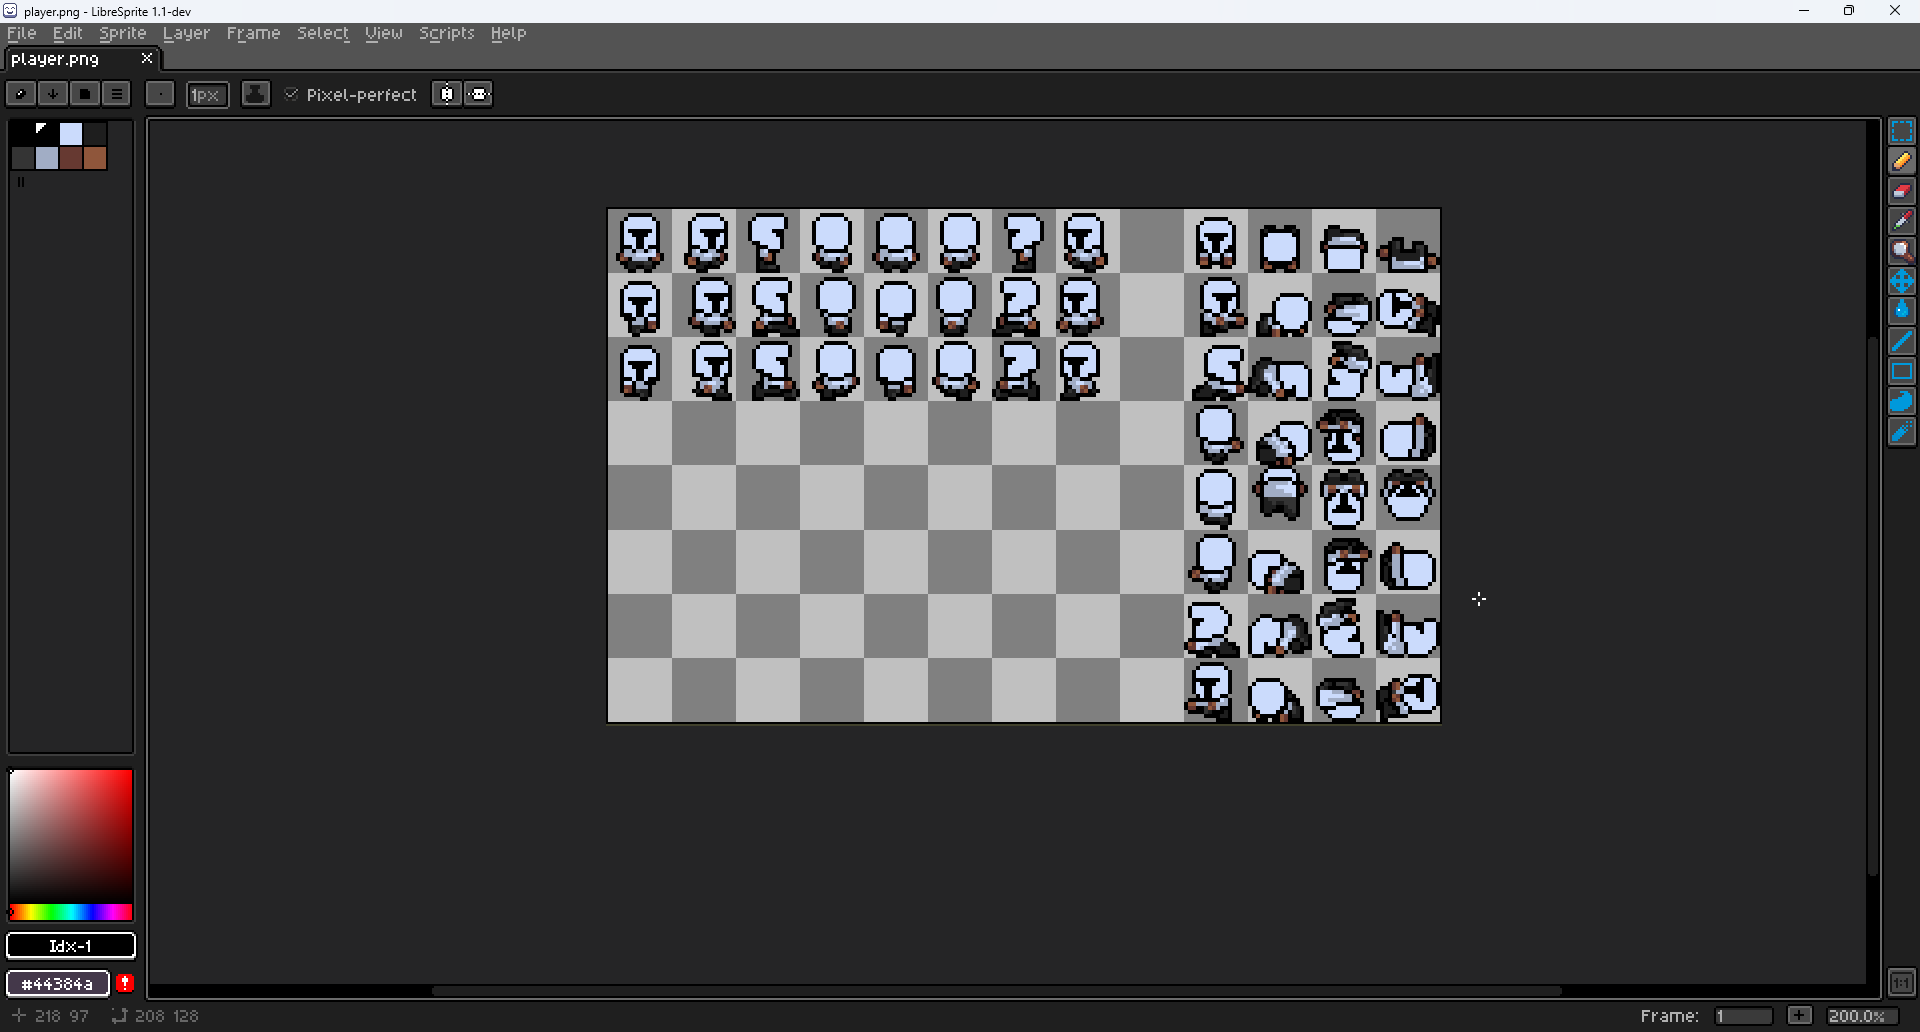
\includegraphics[width=0.9\textwidth]{Figuras/captura_2.png}
\caption{Captura de la interfaz de LibreSprite durante la edición de un \textit{sprite} del juego \textit{Ascension}, mostrando la paleta de colores y el lienzo de edición. \textit{Elaboración propia.}}
\label{fig:placeholder-9}
\end{center}
\end{figure}




\section{Patrones de diseño en el desarrollo de videojuegos}


El desarrollo de videojuegos de complejidad media-alta requiere la aplicación de patrones de diseño (Gamma et al., 1994) \cite{GAMMA_PATTERNS} que faciliten la organización del código, la separación de responsabilidades y la evolución del sistema. A continuación se describen los patrones más relevantes en este contexto, que se han aplicado en el desarrollo de \textit{Ascension}.

\subsection{Patrón \textit{Singleton}}


El patrón \textit{Singleton} establece que una clase disponga de una única instancia en toda la aplicación y proporciona un punto de acceso global a dicha instancia. Su uso implica un compromiso: simplifica el acceso a servicios globales pero introduce un acoplamiento implícito. Se seleccionó el patrón \textit{Singleton} frente a la inyección de dependencias por una razón práctica: en un proyecto individual con cuatro gestores centrales, la infraestructura de un contenedor de inyección de dependencias habría añadido complejidad sin beneficio proporcional. En \textit{Ascension}, se utiliza de forma controlada en los gestores centrales (\textit{GameManager}, \textit{ScoreManager}, \textit{RoomFlowController}, \textit{DamageBoostManager}), todos ellos persistentes entre escenas mediante \texttt{DontDestroyOnLoad}.

\subsection{Patrón \textit{Observer}}


El patrón \textit{Observer} define una relación de dependencia uno-a-muchos entre objetos. Se seleccionó este patrón frente a la alternativa directa -- que el \texttt{GameManager} invocara explícitamente métodos de cada componente de interfaz -- porque esta última habría creado una dependencia inversa que violaría el principio de inversión de dependencias. En \textit{Ascension}, el \textit{GameManager} expone eventos como \texttt{OnGameStateChanged}, \texttt{OnRoomCleared} y \texttt{OnEnemyKilled}, a los que se suscriben los componentes de interfaz de usuario y otros subsistemas.

\subsection{Patrón \textit{Strategy}}


El patrón \textit{Strategy} define una familia de algoritmos, encapsula cada uno de ellos y los hace intercambiables. Se seleccionó frente a la alternativa de una única clase \texttt{Weapon} con condicionales \texttt{if/else}. La clase base \texttt{Weapon} define la interfaz común (método \texttt{Attack()}), mientras que \texttt{MeleeWeapon} y \texttt{RangedWeapon} proporcionan implementaciones específicas. Esto permite añadir nuevos tipos de arma creando una nueva subclase sin modificar el código existente.

\subsection{Patrón \textit{Template Method}}


El patrón \textit{Template Method} define el esqueleto de un algoritmo en una operación, delegando en las subclases la definición de determinados pasos. En \textit{Ascension}, la clase base \texttt{Enemy}  define el ciclo de vida común de todos los enemigos, mientras que las subclases (\texttt{SlimeGreen}, \texttt{SlimeRed}, \texttt{SlimeBlue}) sobrescriben los métodos virtuales para definir su comportamiento específico de IA.

\subsection{Arquitectura basada en componentes (Entidad-Componente)}


Unity se fundamenta en una arquitectura basada en componentes, donde las entidades del juego (\textit{GameObjects}) se definen como contenedores vacíos a los que se agregan componentes (\textit{MonoBehaviour}) que encapsulan funcionalidades independientes. Esta arquitectura favorece la composición sobre la herencia.

\subsection{Máquina de estados (\textit{State Machine})}


Una máquina de estados define un conjunto finito de estados posibles y las transiciones válidas entre ellos. En \textit{Ascension}, el \textit{GameManager} implementa una máquina de estados que controla el flujo global del juego con los estados: \texttt{Menu}, \texttt{CharacterSelection}, \texttt{Playing}, \texttt{Paused}, \texttt{GameOver} y \texttt{Victory}.



\section{Síntesis del estado del arte}


El análisis realizado en este capítulo permite establecer las siguientes conclusiones:

\begin{enumerate}
\item El subgénero \textit{roguelike} presenta retos técnicos de considerable complejidad que justifican su abordaje en un Trabajo de Fin de Grado, incluyendo la generación procedural de contenido, la implementación de inteligencia artificial reactiva y la gestión de múltiples subsistemas en tiempo real. Su creciente relevancia en la industria del videojuego, tanto en términos comerciales como en reconocimiento crítico, refuerza la pertinencia de su estudio.
\item Los títulos comerciales analizados -- \textit{The Binding of Isaac}, \textit{Enter the Gungeon}, \textit{Hades} y \textit{Dead Cells} -- proporcionan referencias de diseño sólidas en cuanto a estructura de niveles, mecánicas de combate, sistemas de enemigos y experiencia de usuario, que se han considerado en el diseño de \textit{Ascension}. El sistema de tiles con efectos constituye un elemento diferenciador del proyecto respecto a las referencias estudiadas.
\item Unity, combinado con el lenguaje C\#, constituye la herramienta más adecuada para el desarrollo del proyecto, dada la madurez de su sistema de \textit{tilemaps}, su soporte para \textit{ScriptableObjects} y la disponibilidad de documentación y recursos.
\item Los patrones de diseño identificados -- \textit{Singleton}, \textit{Observer}, \textit{Strategy} y \textit{Template Method} -- constituyen herramientas fundamentales para la organización del código en proyectos de esta naturaleza y se han aplicado en el desarrollo del proyecto. Adicionalmente, se han empleado mecanismos de estructuración propios del motor (arquitectura basada en componentes) y una máquina de estados para el control del flujo global.
\end{enumerate}












